
\chapter{Bayes minimum risk}
\todo{change notation}

\begin{remark}{Outline}
\todo{outline}
In this chapter, we present the well-known family of \textit{random forests}
methods. In Section~\ref{sec:4:bias-variance}, we first describe the bias-variance
decomposition of the prediction error and then present, in
Section~\ref{sec:4:ensemble}, how aggregating randomized models through
ensembles reduces the prediction error by decreasing the variance term in this
decomposition. In Section~\ref{sec:4:random-forests}, we revisit random forests
and its variants and study how randomness introduced into the decision trees
reduces prediction errors by decorrelating the decision
trees in the ensemble. Properties and features of random forests are then outlined
in Section~\ref{sec:4:features} while their consistency
is finally explored in Section~\ref{sec:4:consistency}.
\end{remark}

\todo{INTRO BMR}

  In this paper two different methods for calibrating probabilities are evaluated and analyzed in 
the context
  of credit card fraud detection, with the objective of finding the model that minimizes the real 
losses due to fraud.
  First, the method proposed \mbox{in \citep{Elkan2001}} to adjust the probabilities based on the 
difference in
  bad rates between the training and testing datasets is used.
  Second, it is compared against the method proposed \mbox{in \citep{Hernandez-Orallo2012}},
  in which calibrated probabilities are extracted after modifying the receiver operating 
characteristic (ROC) curve
  to a convex one using the ROC convex hull methodology.
  
\section{BMR Model}

   We use Bayes minimum risk as a method for cost sensitive credit card fraud detection.
   As defined in \citep{Ghosh2006}, the Bayes minimum risk classifier is a decision model based on
   quantifying tradeoffs between various decisions using probabilities and the costs that accompany 
such decisions.
   In the case of credit card fraud detection, there are two decisions, either predict a 
transaction as fraud $p_f$ or as legitimate $p_l$.
   The risk associated with predicting a transaction as fraud is defined as
   \begin{equation}
    R(p_{f}|x)=L(p_{f}|y_{f})P(p_{f}|x)+L(p_{f}|y_{l})P(p_{l}|x),
    \label{Bayes_min1}
   \end{equation}
   and when the transaction is predicted as legitimate it is
   \begin{equation}
    R(p_{l}|x)=L(p_{l}|y_{l})P(p_{l}|x)+L(p_{l}|y_{f})P(p_{f}|x),
    \label{Bayes_min2}
   \end{equation}
   where %$p_f$ and $p_l$ indicate whether a transaction is predicted as fraud or legitimate, and
   $y_f$ and $y_l$ are the real labels for fraudulent and legitimate transactions respectively. 
$P(p_l|x)$ is the 
   estimated probability of a transaction being legitimate given $x$, similarly 
   $P(p_f|x)$ is the probability of a transaction being fraud given $x$.
   Finally $L(a,b)$ is the loss function when a transaction is predicted as $a$ and the
   real label is $b$.
   Once both risks are calculated, %the decision will be made by choosing the one with the lowest 
cost
   a transaction is classified as fraud if $R(p_{f}|x)\le R(p_{l}|x)$, meaning if the risk 
associated with
   that decision is lower than the risk associated with classifying it as legitimate. % as defined 
in (\ref{Bayes_min3}).
   
   %\noindent 
   Since in the credit card fraud detection case the losses are equal to the cost, first we use 
   the cost matrix with fixed cost for $FN$ as defined in \tablename{ 
\ref{table_measure_cost_hand}}.
   Then a transaction will be classified as fraud if: $C_aP(p_{f}|x)+C_aP(p_{l}|x) \le 
100C_aP(p_{f}|x)$, 
   %the Bayes minimum risk classifier using this cost matrix is defined in (\ref{Bayes_min4}).
   \begin{equation}
    C_aP(p_{f}|x)+C_aP(p_{l}|x) \le 100\cdot C_aP(p_{f}|x),
    \label{Bayes_min4}
   \end{equation}
   and as legitimate otherwise.
  
\section{Calibration of probabilities}

  When using the output of a binary classifier as a basis for decision making,
  there is a need for a probability that not only separates well between 
  positive and negative examples, but that also assesses the real probability of the event 
	\citep{cohen2004}.
  
  In this section two methods for calibrating probabilities are explained.
  First, the method proposed in [6] to adjust the probabilities based on the difference in bad rates
  between the training and testing datasets.
  Then, the method proposed in [8], in which calibrated probabilities are extracted after
  modifying the ROC curve using the ROC convex hull methodology, is described.
  
  \subsection{Brier score and reliability diagrams}
  \todo{Figure of the reliabily diaframs or calibration map}
  
  \subsection{Calibration of probabilities due to a change in base rates.}
  One of the reasons why a probability may not be calibrated is because 
  the algorithm is trained using a dataset with a different base rate than the one on
  the evaluation dataset. 
  This is something common in machine learning since
  using under-sampling or over-sampling is a typical method to solve problems such as
  class imbalance and cost sensitivity \citep{Hulse2007}.
  
  In order to solve this and find probabilities that are calibrated, in \citep{Elkan2001} a formula
  that corrects the probabilities based on the difference of the base rates is proposed.
  The objective is using $p=P(j=1|x)$ which was estimated using a population with base rate 
\mbox{$b=P(j=1)$},
  to find $p'=P'(j=1|x)$ for the real population which has a base rate $b'$.
  A solution for $p'$ is given as follows:
  \begin{equation}
  p'=b'\frac{p-pb}{b-bp+b'p-bb'}.
  \label{cal_prob_br}
  \end{equation}
  Nevertheless, a strong assumption is made by taking: 
  \mbox{$P'(x|j=1)=P(x|j=1)$} and \mbox{$P'(x|j=0)=P(x|j=0)$}, meaning that there
  is no change in the example probability within the positive and negative
  subpopulations density functions.
  
  \subsection{Calibrated probabilities using ROC convex hull.}
  In order to illustrate the ROC convex hull approach proposed in \citep{Hernandez-Orallo2012},
  let us consider the set of probabilities given in \figurename{ \ref{table_example_prob}}.
  Their corresponding  ROC curve of that set of probabilities is shown in \figurename{ 
\ref{ROC_1}}.  It can be seen that this set of probabilities is not calibrated, since at 0.1 there 
is a positive example  followed by 2 negative examples. That inconsistency is represented in the ROC 
curve as a non convex segment  over the curve.
  
  In order to obtain a set of calibrated probabilities, first the ROC curve must be modified in 
order to be convex.
  The way to do that, is to find the convex \mbox{hull \citep{Hernandez-Orallo2012}}, 
  in order to obtain the minimal convex set containing the different points of the ROC curve.
  In \figurename{ \ref{ROC_2}}, the convex hull algorithm is applied to the previously evaluated 
ROC curve.
  It is shown that the new curve is convex, and includes all the points of the previous ROC curve.
  
  Now that there is a new convex ROC curve or ROCCH, the calibrated probabilities can be extracted 
as shown
  in  \figurename{ \ref{cal_prob}}. The procedure to extract the new probabilities is to first group 
the
  probabilities according to the points in the ROCCH curve, and then make the calibrated
  probabilities be the slope of the ROCCH for each group.
  
\begin{figure}[!t]
\hskip 0.5cm
\hbox{
  \vtop{
    \hbox{
      \subfloat[Set of probabilities and their respective class label]{
	\begin{tabular}{cc}
	\hline
	Probability & Label\\
	\hline
	0.0&	0\\
	0.1&	1\\
	0.2&	0\\
	0.3&	0\\
	0.4&	1\\
	0.5&	0\\
	0.6&	1\\
	0.7&	1\\
	0.8&	0\\
	0.9&	1\\
	1.0&	1\\
	\hline
	\end{tabular}\label{table_example_prob}
      }
    }
  }\hskip 0.5cm
  \vtop{\vskip -2.5cm
    \subfloat[ROC curve of the set of probabilities]{
      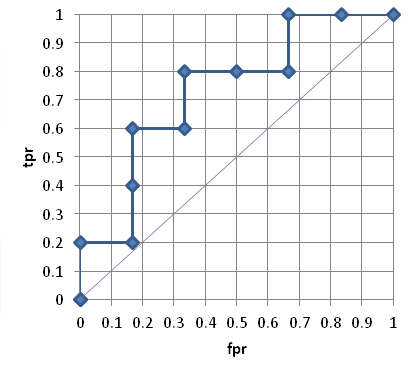
\includegraphics[scale=0.5]{ch6_fig2}\label{ROC_1}
    }%
  }%
}
\vskip 1.5cm

\hbox{ 
  \vtop{ \vskip 0.5cm
    \hbox{
      \subfloat[Convex hull of the ROC curve]{
	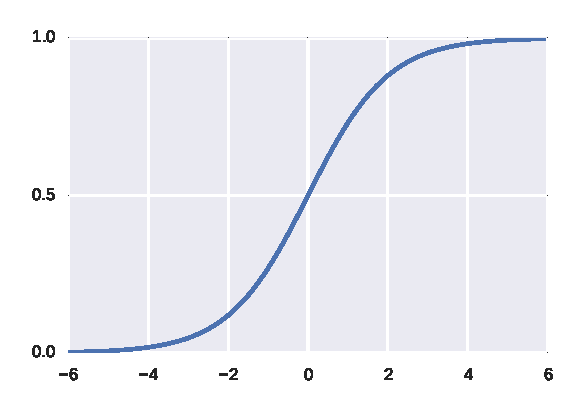
\includegraphics[scale=0.5]{ch6_fig1}\label{ROC_2}
      }
    }
  }\hskip 1cm
  \vtop{ \vskip -1cm
    \subfloat[Calibrated probabilities]{
	\begin{tabular}{cc}
	\hline
	Prob & Cal Prob\\
	\hline
	0.0&	0\\
	0.1&	0.333\\
	0.2&	0.333\\
	0.3&	0.333\\
	0.4&	0.5\\
	0.5&	0.5\\
	0.6&	0.666\\
	0.7&	0.666\\
	0.8&	0.666\\
	0.9&	1\\
	1.0&	1\\
	\hline
	\end{tabular}\label{cal_prob} 
    }
  }
}
\caption{Estimation of calibrated probabilities using the ROC convex hull 
\citep{Hernandez-Orallo2012}.}\label{fig1}

\end{figure}
   
\section{Experiments}
